%Este trabalho está licenciado sob a Licença Atribuição-CompartilhaIgual 4.0 Internacional Creative Commons. Para visualizar uma cópia desta licença, visite http://creativecommons.org/licenses/by-sa/4.0/deed.pt_BR ou mande uma carta para Creative Commons, PO Box 1866, Mountain View, CA 94042, USA.

\chapter{Equações Diferenciais Parciais}\label{cap_edp}
\thispagestyle{fancy}

Neste capítulo, discutimos alguns tópicos fundamentais da aplicação do método de diferenças finitas para a simulação (aproximação da solução) de equações diferenciais parciais.

\section{Equação de Poisson}\label{cap_edp_sec_poisson}\index{equação! de Poisson}

A equação de Poisson em um domínio retangular $D = (x_{\text{ini}}, x_{\text{fin}})\times (y_{\text{ini}}, y_{\text{fin}})$ com condições de contorno de Dirichlet homogêneas refere-se o seguinte problema
\begin{align}
  u_{xx} + u_{yy} &= f(x, y),~(x, y)\in D, \label{eq:edp_Poisson_eq}\\
  u(x_{\text{ini}}, y) &= 0,~y_{\text{ini}}\leq y \leq y_{\text{fin}},\label{eq:edp_Poisson_bcxini}\\
  u(x_{\text{fin}}, y) &= 0,~y_{\text{ini}}\leq y \leq y_{\text{fin}},\label{eq:edp_Poisson_bcxfin}\\
  u(x, y_{\text{ini}}) &= 0,~x_{\text{ini}}\leq x \leq x_{\text{fin}},\label{eq:edp_Poisson_bcyini}\\
  u(x, y_{\text{fin}}) &= 0,,~x_{\text{ini}}\leq x \leq x_{\text{fin}},\label{eq:edp_Poisson_bcyfin}
\end{align}
onde $u = u(x,y)$ é a incógnita.

A aplicação do método de diferenças finitas para resolver este problema consiste dos mesmos passos usados para resolver problemas de valores de contorno (veja Capítulo~\ref{cap_pvc}), a saber: 1. construção da malha, 2. discretização das equações, 3. resolução do problema discreto.

\begin{flushleft}
  {\bf 1. Construção da malha}
\end{flushleft}

Tratando-se do domínio retangular $\overline{D} = [x_{\text{ini}}, x_{\text{fin}}]\times [y_{\text{ini}}, y_{\text{fin}}]$, podemos construir uma malha do produto cartesiano de partições uniformes dos intervalos $[x_{\text{ini}}, x_{\text{fin}}]$ e $[y_{\text{ini}}, y_{\text{fin}}]$. Mais explicitamente, tomamos
\begin{align}
  x_{i} &:= x_{\text{ini}} + (i-1)h_x,\quad h_x = \frac{x_{\text{fin}}-x_{\text{ini}}}{n_x-1},\\
  y_{j} &:= y_{\text{ini}} + (j-1)h_y,\quad h_y = \frac{y_{\text{fin}}-y_{\text{ini}}}{n_y-1},  
\end{align}
onde $i = 1, 2, \dotsc, n_x$, $j = 1, 2, \dotsc, n_y$, sendo $n_x$ e $n_y$ o número de subintervalos escolhidos para as partições em $x$ e $y$, respectivamente.

O produto cartesiano das partições em $x$ e $y$ nos fornece uma partição do domínio $\overline{D}$ da forma
\begin{equation}
  P(\overline{D}) = \{(x_1, y_1), (x_2, y_1), \dotsc, (x_i, y_j), \dotsc, (x_{n_x}, y_{n_y})\},
\end{equation}
cujos nodos $(x_i, y_j)$ podem ser indexados (enumerados) por $k = i + (j-1)n_x$.  Por simplicidade, no decorrer do texto, assumiremos $n_x=n_y=:n$ e, por conseguinte, $h_x=h_y=h$.

\begin{flushleft}
  {\bf 2. Discretização das equações}
\end{flushleft}

Usando a fórmula de diferenças finitas central de ordem $h^2$ para a segunda derivada, temos
\begin{align}
  u_{xx}(x,y) &= \frac{u(x+h,y)-2u(x,y)+u(x-h,y)}{h^2} + O(h^2),\\
  u_{yy}(x,y) &= \frac{u(x,y+h)-2u(x,y)+u(x,y-h)}{h^2} + O(h^2).
\end{align}
Daí, denotando $u_{ij}\approx u(x_i, y_j)$ temos
\begin{align}
  u_{xx}(x_i,y_j) &= \frac{u_{i+1,j}-2u_{i,j}+u_{i-1,j}}{h^2} + O(h^2),\\
  u_{yy}(x_i,y_j) &= \frac{u_{i,j+1}-2u_{i,j}+u_{i,j-1}}{h^2} + O(h^2).  
\end{align}
Então, da equação~\ref{eq:edp_Poisson_eq} temos
\begin{align}
  \frac{u_{i+1,j}-2u_{i,j}+u_{i-1,j}}{h^2} + \frac{u_{i,j+1}-2u_{i,j}+u_{i,j-1}}{h^2} + O(h^2) = f(x_i,y_j).
\end{align}
Adora, denotando $u_k := u_{i+(j-1)n}$, desprezando o termo do erro de truncamento e rearranjando os termos nesta última equação temos
\begin{equation}\label{eq:edp_Poisson_mdf_sis0}
  \frac{1}{h^2}u_{k-n} + \frac{1}{h^2}u_{k-1} -\frac{4}{h^2}u_{k} + \frac{1}{h^2}u_{k+1} + \frac{1}{h^2}u_{k+n} = f(x_i,y_j),
\end{equation}
para $i,j=2, 3, \dotsc, n-1$. Isto é, esta última expressão nos fornece um sistema de $(n-2)^2$ equações para $n^2$ incógnitas $u_k$.

Para fechar o sistema, usamos as condições de contorno \eqref{eq:edp_Poisson_bcxini}-\eqref{eq:edp_Poisson_bcyfin}:
\begin{align}
  u_{1,j} &= 0,\quad u_{n,j}=0,\label{eq:edp_Poisson_mdf_sis1}\\
  u_{i,1} &= 0,\quad u_{i,n}=0\label{eq:edp_Poisson_mdf_sis2},
\end{align}
$i,j=1, 2, \dotsc, n$.

Com isso, o problema discreto obtido da aplicação do método de diferenças finitas consiste no sistema linear de $n^2$ equações \eqref{eq:edp_Poisson_mdf_sis0}-e\eqref{eq:edp_Poisson_mdf_sis2} para as $n^2$ incógnitas $u_k$, $k=1, 2, \dotsc, n^2$.


\begin{flushleft}
  {\bf 3. Resolução do problema discreto}
\end{flushleft}

O problema discreto \eqref{eq:edp_Poisson_mdf_sis0}-e\eqref{eq:edp_Poisson_mdf_sis2} pode ser escrito na forma matricial
\begin{equation}
  A\tilde{u} = b,\label{eq:edp_Poisson_prob_disc}
\end{equation}
onde o vetor da incógnitas é $\tilde{u}=(u_1, u_2, \dotsc, u_{n^2})$ e o vetor dos termos contantes $b$ é tal que
\begin{align}
  i=1,n,~j=1, 2, \dotsc, n &:~b_k = 0,\\
  i=1, 2, \dotsc, n,~j=1,n &:~b_k = 0,\\
  i,j=2, 3, \dotsc, n-1 &:~b_k = f(x_i,y_j).
\end{align}
Além disso, a matriz dos coeficientes $A$ é tal que
\begin{align}
  i=1,n,~j=1, 2, \dotsc, n &:~a_{k,k} = 1,\\
  i=1, 2, \dotsc, n,~j=1,n &:~a_{k,k} = 1,\\
  i,j=2, 3, \dotsc, n-1 &:~a(k,k-n)=\frac{1}{h^2},\\
                        &~~a(k,k-1)=\frac{1}{h^2},\\
                        &~~a(k,k)=-\frac{4}{h^2},\\
                        &~~a(k,k+1)=\frac{1}{h^2},\\
                        &~~a(k,k+n)=\frac{1}{h^2}.
\end{align}
Assim sendo, basta empregarmos um método apropriado para resolver o sistema linear \eqref{eq:edp_Poisson_prob_disc} para obter a solução aproximada de $u$ nos nodos $(x_i, y_j)$.


\begin{ex}\label{ex:edp_Poisson}
  Consideremos o seguinte problema
  \begin{align}
    u_{xx} + u_{yy} &= -\sen(x)\sen(y),~(x, y)\in (0, \pi)\times (0, \pi),\\
    u(0, y) &= 0,~y\in [0, \pi],\\
    u(\pi, y) &= 0,~y\in [0, \pi],\\
    u(x, 0) &= 0,~x\in [0, \pi],\\
    u(x, \pi) &= 0,~x\in [0, \pi].
\end{align}


\begin{figure}[h!]
  \centering
  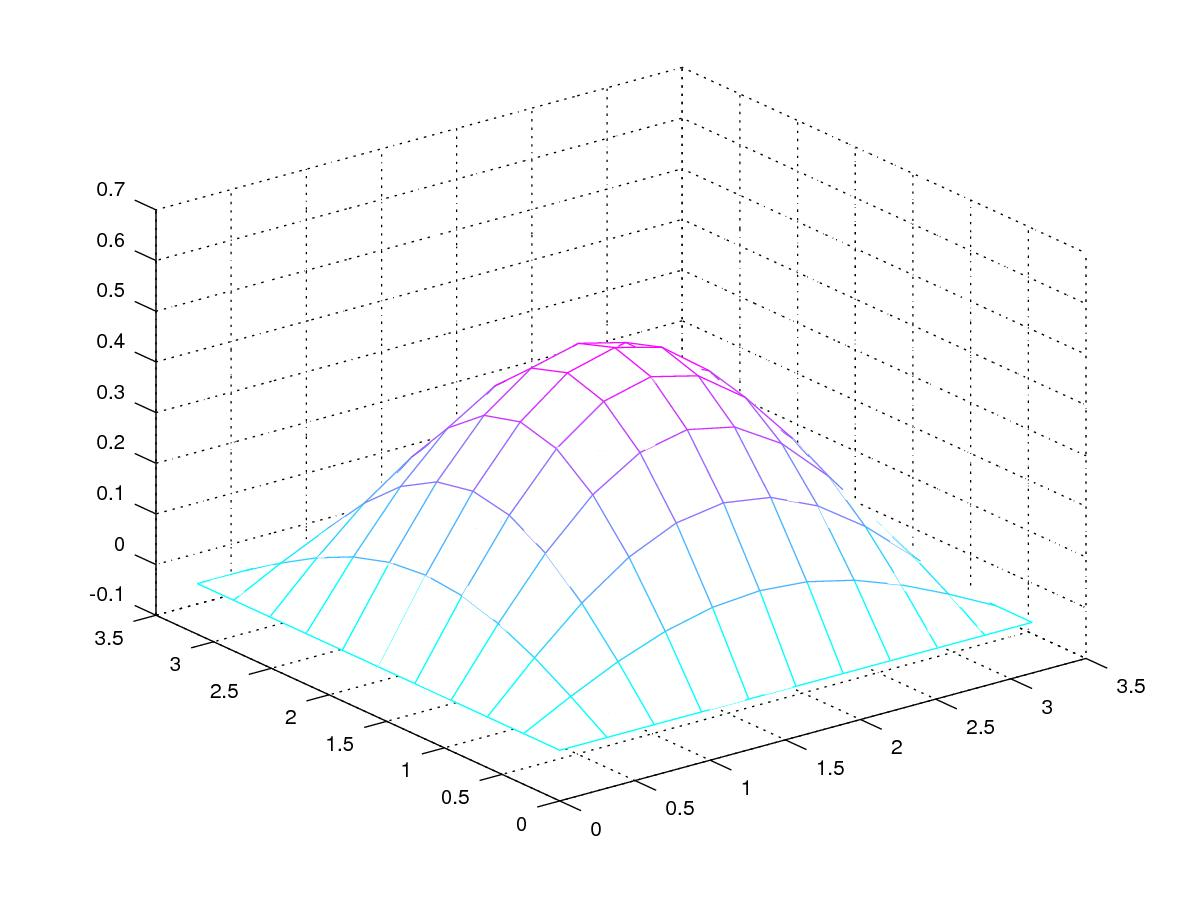
\includegraphics[width=0.8\textwidth]{./cap_edp/dados/ex_edp_Poisson/ex_edp_Poisson}
  \caption{Resultado referente ao Exemplo~\ref{ex:edp_Poisson}.}
  \label{fig:ex_edp_Poisson}
\end{figure}


A Figura~\ref{fig:ex_edp_Poisson} mostra um esboço do gráfico da solução aproximada obtida pelo método de diferenças finitas apresentado acima (equações \eqref{eq:edp_Poisson_mdf_sis0}-\eqref{eq:edp_Poisson_mdf_sis2}) com $n=11$, i.e. $h=\pi/10$.

\begin{table}[h!]
  \centering
  \begin{tabular}{l|c}
    $n$ & $\|\tilde{u}-u\|_{L^2}$\\\hline
    $6$ & $4,2\E-2$ \\
    $11$ & $2,1\E-2$ \\
    $21$ & $1,0\E-2$ \\
    $41$ & $5,1\E-3$ \\
    $81$ & $2,6\E-3$ \\\hline
  \end{tabular}
  \caption{Resultados referentes ao Exemplo~\ref{ex:edp_Poisson}.}
  \label{tab:ex_edp_Poisson}
\end{table}

Na Tabela~\ref{tab:ex_edp_Poisson} temos a norma $L^2$ da diferença entre a solução aproximada $\tilde{u}$ e a solução analítica $u(x,y) = 0,5\sen(x)\sen(y)$ nos pontos de malha computados com diferentes escolhas de $n$.

\ifisoctave
Os resultados obtidos neste exemplo podem ser obtidos no \verb+GNU Octave+ com o seguinte código:
\begin{verbatim}
#params
n=11;
h=pi/(n-1);

#fonte
f = @(x,y) -sin(x).*sin(y);

#malha
x = linspace(0,pi,n);
y = linspace(0,pi,n);

#sistema MDF
A = zeros(n*n,n*n);
b = zeros(n*n,1);

#cc x=0 e x=pi
for i=[1,n]
  for j=1:n
    k = i + (j-1)*n;
    A(k,k)=1;
    b(k) = 0;
  endfor
endfor

#cc y=0, y=pi
for j=[1,n]
  for i=1:n
    k = i + (j-1)*n;
    A(k,k)=1;
    b(k) = 0;
  endfor
endfor

#nodos internos
for i=2:n-1
  for j=2:n-1
    k = i + (j-1)*n;
    A(k,k-n) = 1/h^2;
    A(k,k-1) = 1/h^2;
    A(k,k) = -4/h^2;
    A(k,k+1) = 1/h^2;
    A(k,k+n) = 1/h^2;
    
    b(k) = f(x(i),y(j));
  endfor
endfor

u = A\b;

#visu
z = zeros(n,n);
for i=1:n
  for j=1:n
    k = i + (j-1)*n;
    z(i,j) = u(k);
  endfor
endfor
colormap("cool")
mesh(x,y,z)

ua = zeros(n*n,1);
for i=1:n
  for j=1:n
    k=i+(j-1)*n;
    ua(k) = 0.5*sin(x(i))*sin(y(j));
  endfor
endfor
printf("%d %1.5E %1.1E\n",n,h,norm(u-ua))
\end{verbatim}
\fi
\end{ex}

\subsection*{Exercícios}

\emconstrucao

\section{Equação do calor}\label{cap_edp_sec_calor}\index{equação!do calor}

\emconstrucao

\section{Equação da onda}\label{cap_edp_sec_onda}\index{equação!da onda}

\emconstrucao